\section{Problem in Neural Network}
\label{sec:Problem}

Though neural network is able to achieve numerous back breaking tasks, it is 
fairly challenging to well train a neural network. Among all the difficulties,
gradient explosion and vanishing is the most famous one. In this section, we
will discuss a few problems in training a neural network.

\subsection{Explosion and Vanishing}
Intuitively, using the computation like 
$ Z^{[l]} = W^{[l]}A^{[l-1]} $ and 
$ dA^{[L-1]} = W^{[L-1]T}dZ^{[L]} $ in FP and BP, if $ W $ is much larger 
than 1 or much smaller than 1, after several multiplication in the deep 
neural network the final result $ Z^{[l]} = \prod\limits_{l=1}^LW^{[l]}A^{[0]} $
will gradually tend to be infinity or zero. Here we further illustrate 
the explosion and vanishing with a simple problem from \parencite{shamir2018exponential}:

\begin{exmp}
    Suppose there is only one parameter $ w $.
    for a data set $\{x,\ y\}$ and a special architecture, 
    the cost function is:
    \begin{equation}
        J(w) = (w^7 + 1)^2
    \end{equation}
    The plot of $J(w)$ is illustrated in \autoref{fig:exmp1}. The global
    minimum $ w^* = -1 $, a basin exists in the region of $ [-1.05,\ -0.95] $.
    But in the region of $ [-\infty,\ -1.05],\ [1.05,\ \infty] $, $ J(w) $
    is extremely steep, which is the explosion, and in the region of 
    $ [-0.95,\ 1.05] $, $ J(w) $ is unusually flat, which is the vanishing.
    If the initial value $ w_0 $ falls into the basin, GD will converge 
    quickly. If not, let's say $ w_0 = 0.5 $, then it would be terrible to
    traverse through the plateau with a tiny update in each iteration.
\end{exmp}

\begin{figure}[H]
    \centering
    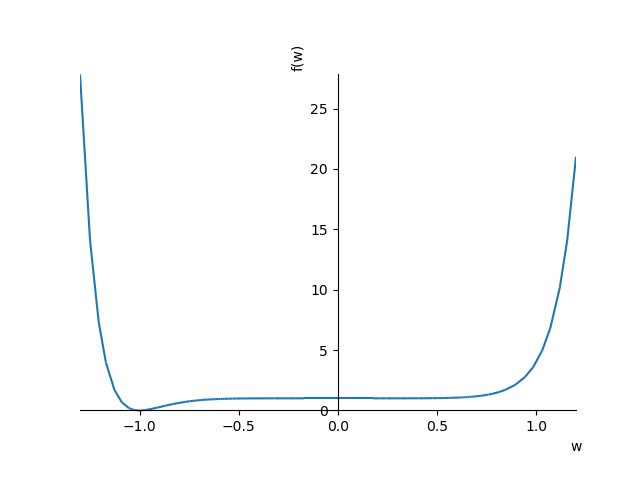
\includegraphics[width=10cm]{exmp1}
    \caption{\label{fig:exmp1}Plot of $ J(w) = (w^7 + 1)^2 $}
\end{figure}

\subsection{Saddle Points in Non-convex Optimization}
Though there seems to be no rigorous proof of the prevalence of saddle points 
in high dimensional non-convex optimization, one line of the evidence 
is carried out astonishingly from statistical physics. It suggests that 
among a myriad of critical points, most are likely to be saddle points.
To understand the landscape in the neural network optimization, we first
introduce the Hessian Matrix to pave the way for further discussion.

\subsubsection{Hessian Matrix}
\begin{defn}
    \label{def:Hessian}
    Suppose $ f: \mathbb{R}^n\rightarrow R $, all second partial derivatives
    of $ f $ exist and are continuous over the domain. The Hessian Matrix 
    $ \mathbf{H} \in \mathbb{R}^{n\times n} $ of $ f $ is defined and arranged
    as follow:
    \begin{equation}
        \mathbf{H} =
        \begin{pmatrix}
            \frac{\partial^2f}{\partial x_1^2} & \frac{\partial^2f}{\partial x_1\partial x_2} & \cdots & \frac{\partial^2f}{\partial x_1\partial x_n} \\
            \frac{\partial^2f}{\partial x_2\partial x_1} & \frac{\partial^2f}{\partial x_2^2} & \cdots & \frac{\partial^2f}{\partial x_2\partial x_n} \\
            \vdots & \vdots & \ddots & \vdots \\
            \frac{\partial^2f}{\partial x_n\partial x_1} & \frac{\partial^2f}{\partial x_n\partial x_2} & \cdots & \frac{\partial^2f}{\partial x_n^2}
        \end{pmatrix}
    \end{equation}
    If the second partial derivatives are continuous, then the order of partial
    derivatives does not matter. Thus, $ \mathbf{H} $ is a symmetric matrix.
\end{defn}

\par Since the Hessian Matrix is symmetric, the eigenvalues are real numbers,
i.e. $ \lambda_i \in R $. For a cost function $ J(\theta) $, where 
$ \theta \in \mathbb{R}^n $ represents the high dimensional variable. The 
properties of critical points\footnote{Critical points are points 
$ \theta $ where $ \nabla J(\theta) = 0 $. } can be described by the eigenvalues
of the Hessian.
\begin{enumerate}
    \item If $ \forall \lambda_i \in R^+ $, i.e. Hessian is positive definite, then the critical point is a local minimum.
    \item If $ \forall \lambda_i \in R^- $, i.e. Hessian is negative definite, then the critical point is a local maximum.
    \item If $ \forall \lambda_i \neq 0 $, some are positive and others are negative,
        then the critical point is a (horse) saddle point with min-max structure.
    \item If Hessian matrix is singular, i.e. $ |\mathbf{H}| = 0 $, then
        the critical point is called degenerate critical point and it is 
        a monkey saddle point. 
\end{enumerate}

\begin{figure}[ht]
    \centering
    \subfigure[local minimum]{
        \begin{minipage}[t]{0.5\linewidth}
        \centering
        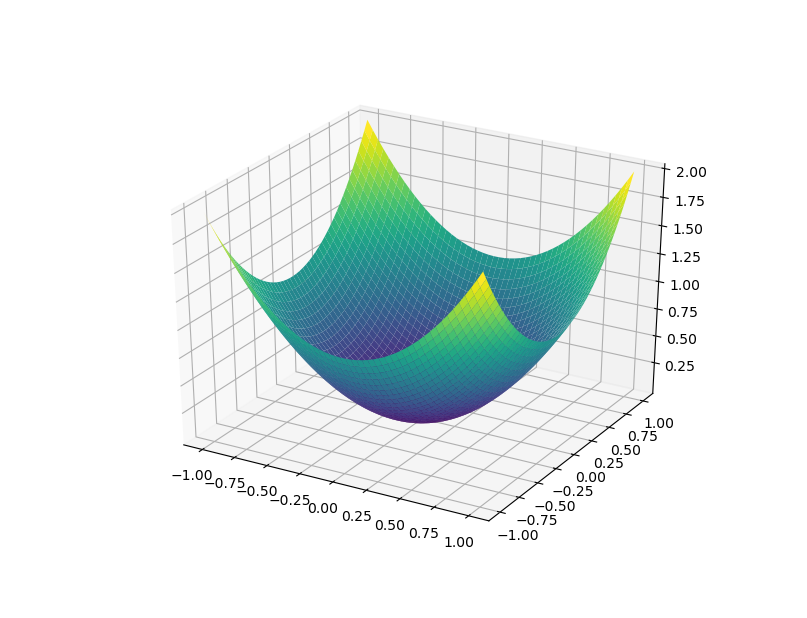
\includegraphics[width=6cm]{minimum.png}
        \end{minipage}%
    }%
    \subfigure[local maximum]{
        \begin{minipage}[t]{0.5\linewidth}
        \centering
        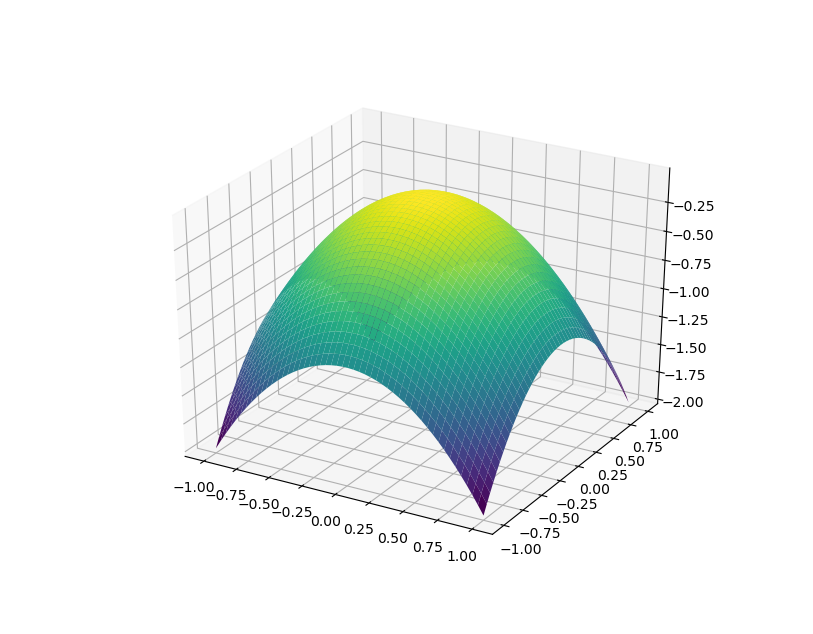
\includegraphics[width=6cm]{maximum.png}
        \end{minipage}%
    }%

    \subfigure[horse saddle point]{
        \begin{minipage}[t]{0.5\linewidth}
        \centering
        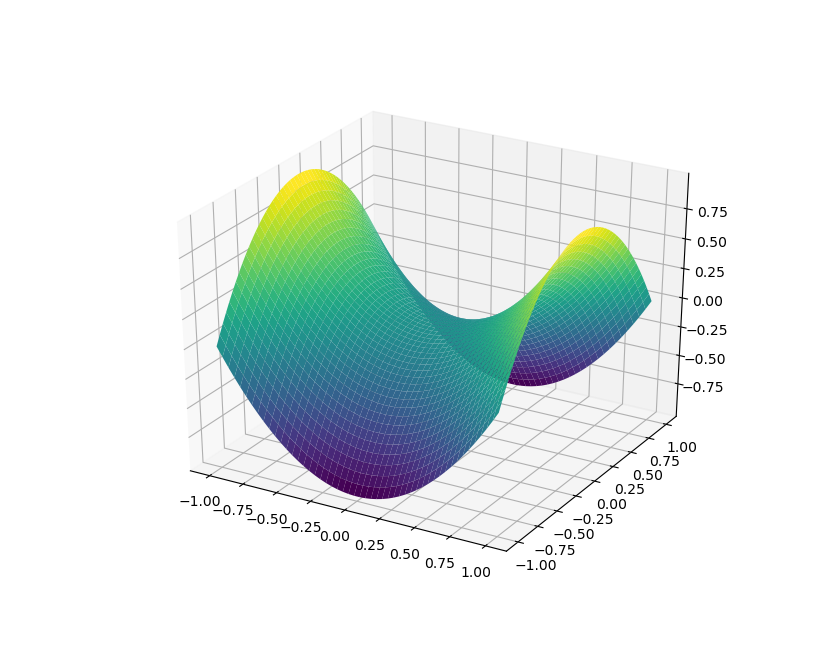
\includegraphics[width=6cm]{horse.png}
        \end{minipage}%
    }%
    \subfigure[monkey saddle point]{
        \begin{minipage}[t]{0.5\linewidth}
        \centering
        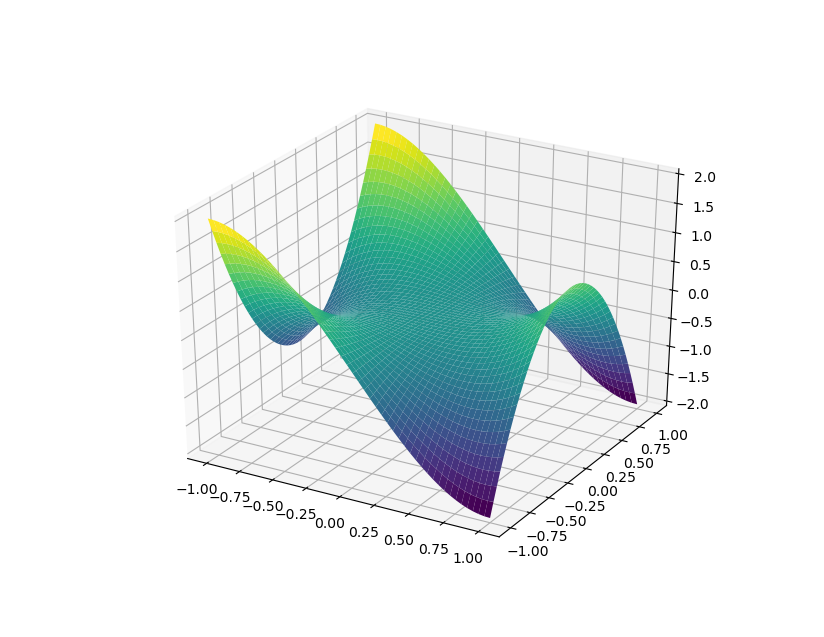
\includegraphics[width=6cm]{monkey.png}
        \end{minipage}%
    }%
    \centering
    \caption{\label{fig:activation}Different types of critical point}
\end{figure}

\subsubsection{The Prevalence of Saddle Points}
\label{sssec:Saddle}
In the early version of neural network algorithms, parameters are initialized
with standard Gaussian noise. The article by Bray et al. \parencite{bray2007statistics}
computes the average number of critical points of a Gaussian distribution
on a high dimensional space. They derive the distribution of critical points
with a relation between $ \alpha $ and $ \epsilon $, where $ \alpha $ is
the fraction of negative eigenvalues of the Hessian at the critical points, 
$ \epsilon $ is the error at the critical points. In a Gaussian field $ \phi $
defined over volume $ V $ of an N-dimensional Euclidean space. The normalized
density of eigenvalues defined as:
\begin{equation}
    \rho(\lambda) = \frac{1}{N}\sum\limits_{i=1}^N\delta(\lambda-\lambda_i)
\end{equation}
The average of eigenvalues is defined as:
\begin{equation}
    \bar(\lambda)=\int \lambda\rho(\lambda) d\lambda
\end{equation}
And it can be computed via:
\begin{equation}
    \bar{\lambda}(\epsilon)=2 \frac{f^{\prime}(0) \epsilon}{f^{\prime \prime}(0) P}
\end{equation}
where $ P $ is defined as follow:
\begin{equation}
    P=\frac{f^{\prime}(0)^{2}}{f^{\prime \prime}(0)^{2}}+\frac{f(0)}{f^{\prime \prime}(0)}\left(1-\frac{2}{N}\right) \approx \frac{f^{\prime}(0)^{2}}{f^{\prime \prime}(0)^{2}}+\frac{f(0)}{f^{\prime \prime}(0)}
\end{equation}
Finally, the relation between $ \alpha $ and $ \epsilon $ is given by:
\begin{equation}
    \frac{2}{\pi} \int_{\frac{\bar{\lambda}}{2 \sqrt{f^{\prime \prime}(0)}}}^{1} (1-u^{2})^{\frac{1}{2}}du=\alpha
\end{equation}
where $ u $ just a temporary variable in the integration computation. 
\par In the $ \epsilon-\alpha $ graph, there is a global minimum at 
$ \alpha = 0,\ \epsilon = \epsilon_{min} $ and 
a global maximum at $ \alpha = 1,\ \epsilon = \epsilon_{max} $. Other 
critical points a located on a monotonically increasing curve as $ \alpha $
ranges from 0 to 1. Some experiments validating such proposal is finished 
by Dauphin et al. \parencite{dauphin2014identifying} in \autoref{fig:aevalidation}.
This implies that local minimums, i.e. critical points
that $ \alpha\rightarrow 0 $, are more closer to global minimum, while 
the majority of critical points that have high error are likely to have 
a large percentage of negative eigenvalues, i.e. most of critical points 
are saddle points.

\begin{figure}[H]
    \centering
    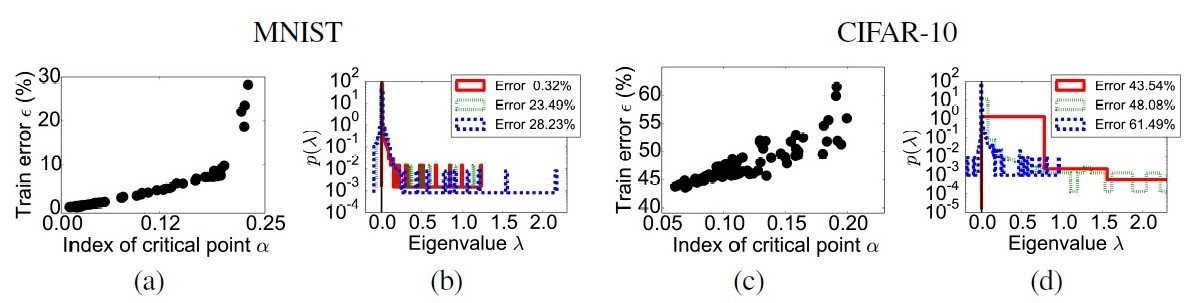
\includegraphics[width=14cm]{aevalidation}
    \caption{\label{fig:aevalidation}(a) and (c) show how critical points 
    are distributed in the $ \epsilon-\alpha $ plane. (b) and (d) plot the 
    distributions of eigenvalues of the Hessian at three different 
    critical points.}
\end{figure}

\subsection{Learning Rate Selection}
The choice of stepsize has long been a puzzle to practitioners in neural
networks. In fact, it is not peculiar to GD but a common problem in optimization.
If the learning rate is too large, with high probability GD will diverge. If
learning rate is too small, the time GD takes to converge is unbearable.
In practice, the most widely used scheme is setting learning rate as a small
constant like 0.1 or 0.01. The drawback of such scheme is obvious: it does not
guarantee the convergence of GD. 
\par First we review the general optimization problem:
\begin{align*}
    x_{k+1} = x_{k} - \alpha_k d_k
\end{align*}
We list other commonly used scheme in the following.

\subsubsection{Goldstein Rule}
Goldstein rule is the first effective rule for stepsize selection in 
general optimization problem that does not depend on linear minimization. 
Let $ \sigma \in (0,\ 0.5),\ \alpha_k $ satisfied:
\begin{equation}
    \sigma \leq \frac{f\left(x^{k}+\alpha^{k} d^{k}\right)-f\left(x^{k}\right)}{\alpha^{k} ||d^{k}||^2} \leq 1-\sigma
\end{equation}

\subsubsection{Armijo Rule}
\label{sssec:Armijo}
It is natural to devise a scheme that successively reduce $ \alpha $, when 
$ f(x_{k+1}) < f(x_k) $ is not satisfied. The Armijo rule is exactly based
on the this devisal. Here, let $ s \in R,\ \beta,\ \sigma \in [0,\ 1],\ 
\alpha_k=\beta^{m_k}s $, where $ m_k $ is the first nonnegative integer
satisfies:
\begin{equation}
    f(x_{k}) - f(x_{k} - \beta^{m_k}sd_k) \geq -\sigma\beta^{m_k}s\nabla ||d_k||^2
\end{equation}
\par Usually $ \sigma \in [10^{-5},\ 10^{-1}],\ \beta \in [0.1,\ 0.5],\ s=1 $.

\subsubsection{Diminishing Learning Rate}
During the process of optimization, we let $ \alpha_k\rightarrow 0 $.
The primary downside of such scheme is that after multiple iterations
the stepsize may be too small to descent. So an additional requirement
is added:
\begin{equation}
    \sum\limits_{k=0}^\infty\alpha_k = \infty
\end{equation}
